\chapter{Theoretical Background}
\label{ch:theoretical_background}

\section{Dynamical Systems and Tipping Points}
A dynamical system is any system whose state changes over time by following a fixed rule. In this thesis the ``state'' is a chemical measurement taken from a sediment core -- for example, the amount of molybdenum or barium at a certain depth. The ``rule'' is the physics and chemistry of the ancient Mediterranean Sea that decided what that amount would be. We can never see the rule itself. We only see the long list of measurements it produced, going down the core, and the job is to learn something about the hidden rule from that list.

The easiest way to picture this is a ball rolling inside a landscape of hills and valleys. The bottom of a valley is a stable state: push the ball a little and it rolls back down. The top of a hill is an unstable state: push the ball a little and it rolls away and does not come back. A real system is never left alone. It is always being pushed around by small random disturbances -- for the Mediterranean, think of normal changes in weather from one year to the next. So the ball is always being knocked part way up the valley wall and always rolling back down again.

Written as an equation, a system with one changing value $x$ follows $\frac{dx}{dt} = f(x)$. This says that the speed at which $x$ changes depends on the current value of $x$, through some function $f$. An equilibrium is a value $x^*$ where the system stops changing, which means $f(x^*) = 0$ -- the ball is standing still. Whether that point is a valley or a hilltop depends on the slope of $f$ there. If the slope is negative ($f'(x^*) < 0$), a small move away creates a push back toward $x^*$, so it is a valley (stable). If the slope is positive ($f'(x^*) > 0$), a small move away grows instead of shrinking, so it is a hilltop (unstable).

Now let the shape of the landscape slowly change, because some outside condition is slowly drifting -- for the Mediterranean, this is the slow change in Earth's orbit that changes the strength of the monsoon over tens of thousands of years. Call that slowly drifting condition $\lambda$. The equation becomes $\frac{dx}{dt} = f(x, \lambda)$. As $\lambda$ moves, the hills and valleys move too: a valley can grow deeper, grow shallower, or flatten out. A tipping point is a specific value $\lambda_c$ where the landscape does not just change a little, but changes in kind: a valley the ball was sitting in flattens out completely and disappears. Once that valley is gone, nothing holds the ball in place, and it rolls quickly to a far-away part of the landscape and settles there instead. This roll-away is fast, it is large, and pushing $\lambda$ back a little does not bring the old valley back. In mathematics this moment -- a valley or hill appearing, disappearing, or trading places -- is called a bifurcation. ``Tipping point'' is the term used in climate science and ``bifurcation'' is the exact mathematical term for the same event; the rest of this chapter uses the mathematical one. For this thesis, the tipping event is the start of a sapropel: the deep water of the Mediterranean switching from oxygen-rich to oxygen-starved, which the sediment records as a sharp jump in molybdenum and a few other chemical markers.

\section{Bifurcation Theory and Normal Forms}
\label{sec:normal_forms}
A real system like the Mediterranean has many interacting parts, far too many to capture in a single equation. What lets us still say something simple is a mathematical result called the Center Manifold Theorem. It says that when a system is close to a tipping point, almost all of its parts are still firmly stable and settle back quickly if disturbed; only one or two are close to losing their grip. Those one or two slow parts control what happens at the tipping point, and everything else can be set aside. So a system with many variables behaves, right at the edge of tipping, like a system with just one or two.

That reduced system always takes one of a few standard forms, called normal forms \citep{kuznetsov2004,strogatz2015}. This thesis uses three: the Fold, the Transcritical, and the Hopf bifurcation, each a different way for a stable state to be lost. One caveat matters for later chapters: the synthetic data this thesis trains on is not built from these three bare equations, but from a large set of randomly-built systems, each checked to pass through one of these three bifurcation types near its own tipping point (Chapter~\ref{ch:data}, Section~\ref{sec:sde_corpus}). The normal forms still describe them all, because the Center Manifold Theorem guarantees it.

\subsection{The Fold Bifurcation}
The Fold bifurcation (also called the saddle-node bifurcation) is the standard model for a sudden, one-way jump. It is the type most often used to describe the collapse of ocean circulation, and the onset of an anoxic sapropel. Its simplest form is $\frac{dx}{dt} = \lambda - x^2$. Setting the right side to zero, the equilibria are $x^* = \sqrt{\lambda}$ and $x^* = -\sqrt{\lambda}$, which only exist when $\lambda > 0$. The one at $x^* = \sqrt{\lambda}$ is a valley (stable); the one at $x^* = -\sqrt{\lambda}$ is a hilltop (unstable). As $\lambda$ slowly falls toward zero, the valley and the hilltop slide toward each other. At $\lambda = 0$ they meet and cancel out. For any $\lambda < 0$ there is no equilibrium here at all -- the valley is simply gone, and the system slides away to some far-off state. Because the valley does not come back when $\lambda$ rises slightly again, the jump is effectively permanent. This is what makes the Fold the ``catastrophic'' case. A real-world example is a shallow lake that stays clear for years while nutrient pollution slowly builds up, then flips within a single season into a permanently green, algae-choked state that does not clear again even if the pollution is later reduced \citep{scheffer2009}.

\subsection{The Transcritical Bifurcation}
The Transcritical bifurcation is gentler. Instead of a valley and a hilltop meeting and vanishing, two equilibria pass through each other and swap which one is stable. Its simplest form is $\frac{dx}{dt} = \lambda x - x^2$, with equilibria at $x^* = 0$ and $x^* = \lambda$. When $\lambda > 0$, the point $x^* = \lambda$ is the valley and $x^* = 0$ is the hilltop. As $\lambda$ passes through zero, they cross, and afterwards $x^* = 0$ is the valley and $x^* = \lambda$ is the hilltop. The key difference from the Fold is that there is always a valley somewhere for the system to sit in -- it just moves, and the system tracks it smoothly, without a sudden jump to somewhere distant. A real-world example is a species newly arriving in a habitat: under poor conditions its population always shrinks back to zero, but once conditions cross a threshold, a small founding population instead grows and establishes itself -- the ``absent'' and ``established'' states trade stability, with no sudden jump.

\subsection{The Hopf Bifurcation}
The Hopf bifurcation cannot happen in a one-variable system, because it involves the system starting to go round in circles, and a single number cannot turn. It needs at least two variables. Written using a radius $r$ (distance from the resting state) and an angle $\theta$ (position around the circle), its simplest form is $\frac{dr}{dt} = \lambda r - r^3$, $\frac{d\theta}{dt} = \omega$. When $\lambda < 0$, the only equilibrium is $r^* = 0$: the system sits still. As $\lambda$ crosses zero, that resting state becomes unstable, and instead the system settles into a steady loop of radius $r^* = \sqrt{\lambda}$, going round at rate $\omega$. This steady loop is called a limit cycle. In a real time series, a Hopf bifurcation shows up as an oscillation that appears and grows as the tipping point is approached. A real-world example is a predator and prey pair whose numbers settle to steady values under some conditions, but past a threshold begin a repeating boom-and-bust cycle instead. This growing oscillation is a feature the other two bifurcations do not have, which (as the next section explains) makes the Hopf the easiest of the three for a classifier to pick out.

\begin{figure}[htbp]
    \centering
    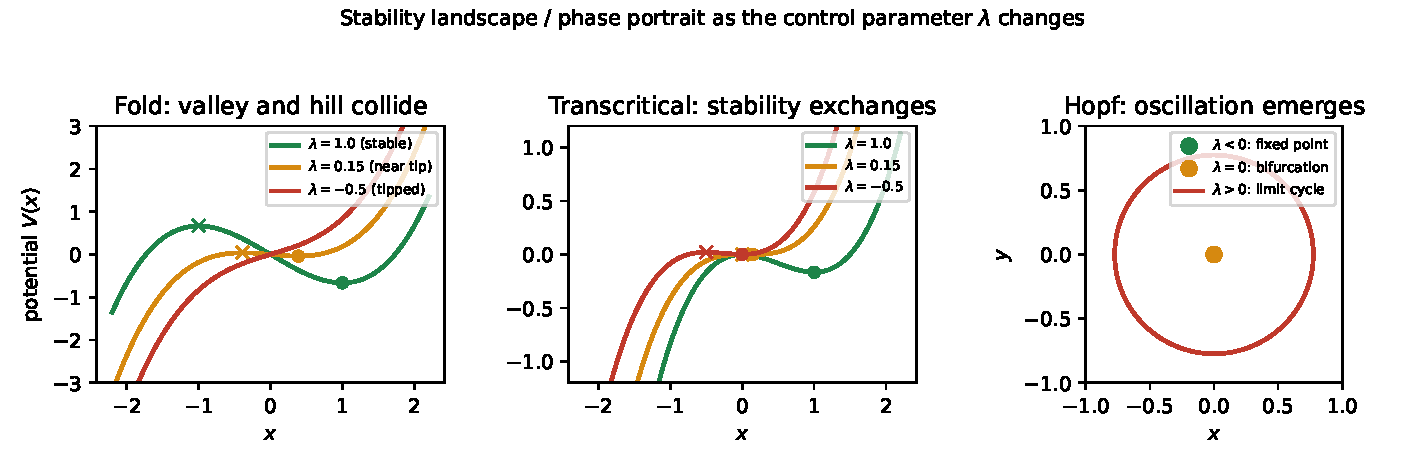
\includegraphics[width=0.98\textwidth]{figures/fig3_bifurcation_landscapes.pdf}
    \caption{The stability landscape (or phase portrait, for Hopf) for each bifurcation as $\lambda$ moves toward its critical value. Fold: the stable point (circle) and unstable point (cross) move together and vanish. Transcritical: the two equilibria cross and swap stability. Hopf: the fixed point gives way to a stable oscillating orbit.}
    \label{fig:3_1}
\end{figure}

\subsection{Why Fold and Transcritical Are Hard to Tell Apart}
\label{sec:fold_transcritical_challenge}
Of the three bifurcation types, the Hopf is the easy one to spot. It produces a growing oscillation before the tipping point, and neither of the other two does anything like that, so an oscillation appearing in the data is a strong hint that a Hopf is coming.

The Fold and the Transcritical are the hard pair. On the approach to the tipping point, both show the same two things in the data: the variance rises and the lag-1 autocorrelation rises (the next section explains why). There is no oscillation, no obvious shape, nothing to separate them by eye. And yet the two matter for very different reasons: a Fold is a sudden, permanent jump to a far-off state, while a Transcritical is a smooth, controlled shift. Telling a real record that it is heading for a Fold when it is actually heading for a Transcritical would be a serious mistake for an early-warning system.

The difference is there in the equations, just not in a form the raw data shows directly. For the Fold, the stable state sits at $x^* = \sqrt{\lambda}$, so as $\lambda$ shrinks the state moves like the square root of the distance to the tipping point -- slowly at first, then faster and faster. For the Transcritical, the stable state sits at $x^* = \lambda$, so it moves in simple proportion to the distance -- at a steady rate. This carries over to the variance: for the Fold, the variance does not just rise, it rises at an accelerating rate; for the Transcritical, it rises steadily. The rate of rise, not the rise itself, is what separates them.

A classifier looking only at the raw series, or at the raw variance, has to work this rate difference out on its own, from noisy data, which is hard. This thesis instead hands the classical (non-deep-learning) models in its roster the accumulated growth directly, as an extra input channel called the variance growth ratio: at each point along the record it divides the current windowed variance by the windowed variance measured at the start, then takes $\log(1+\cdot)$ so the channel stays on a manageable scale (Chapter~\ref{ch:data}, Section~\ref{sec:feature_engineering} defines it exactly, and states precisely which models receive it). The deep-learning models in the roster are not given this channel; they read the raw series directly and have to learn any such distinction themselves. Because a Fold's variance accelerates while a Transcritical's grows steadily, this ratio climbs faster and curves upward more sharply for a Fold, so the rate difference of the previous paragraph is present in the channel as a difference in shape the model can read off, rather than a derivative it has to estimate from noise. Before treating this as an original construction, I checked whether it already exists in the closest prior work. It does not appear in \citet{bury2021}, and it does not appear in their 2023 follow-up on classifying bifurcation type \citep{bury2023discretetime}, which I confirmed by reading its methods section directly -- that paper feeds only the raw normalised series into its classifier, with no engineered variance-growth channel of any kind. A broader (though not exhaustive) search found no other paper doing this, so it is reported here as this thesis's own construction.

\section{Critical Slowing Down (CSD)}
\label{sec:csd}
We cannot observe the stability landscape directly. What we have is the data the system left behind -- for this thesis, a column of chemical measurements down a sediment core. Critical Slowing Down is the effect that connects the two: as a system moves toward a tipping point, it recovers more and more slowly from small disturbances, and this slowdown leaves a measurable trace in that data. It is what every method in this thesis is trying to detect.

The reason for the slowdown is that the ``valley'' holding the system in place becomes shallower as the tipping point nears, so the pull back toward the resting state weakens. A useful way to state this is through the recovery time: the time a small disturbance takes to fade. Far from a tipping point the recovery time is short; as the tipping point is approached it grows longer and longer, and in the limit it becomes infinite.

This slowdown produces two changes in a recorded time series, and these two are the classic early warning signals:

\textbf{Rising variance.} With a weaker pull back toward the resting state, ordinary random disturbances carry the system further from that state before it returns. The recorded values spread out over a wider range, so their variance increases.

\textbf{Rising lag-1 autocorrelation.} With a slower recovery, each value in the record is more strongly influenced by the value just before it -- the previous disturbance has not yet faded. The correlation between each measurement and the one immediately preceding it therefore rises, approaching its maximum of 1.

Both quantities can be computed directly from a real sediment core even though the equations governing the core cannot. Detecting a rise in them, or detecting something more informative, is the task of the rest of this thesis.

\section{The AR(1) Model}
\label{sec:ar1_model}
A real sediment core is a bumpy, noisy record, not a smooth line, and it comes as a list of separate measurements taken step by step down the core. The simplest standard way to describe data like this -- a value that gets randomly pushed around but keeps coming back to a normal level -- is a model called AR(1) (short for ``autoregressive model of order one''): $y_{t+1} = \alpha\, y_t + \epsilon_t$. This just says: the next value ($y_{t+1}$) equals some fraction $\alpha$ of the current value ($y_t$), plus a new random amount ($\epsilon_t$) added each step that has nothing to do with the previous one. The fraction $\alpha$ is a number between 0 and 1. It is the same lag-1 autocorrelation from the previous section: it says how much of each value is carried over into the next one. If $\alpha$ is small, most of each value is fresh randomness, and the series comes back to its normal level quickly. If $\alpha$ is close to 1, almost the whole value is carried over, so the series can drift a long way from its normal level and take a long time to come back. This is exactly what Critical Slowing Down does, so $\alpha$ climbs toward 1 as a tipping point gets close.

How spread out the values are also follows a simple rule. If the random amounts added each step have a spread (variance) of $\sigma_\epsilon^2$, then the spread of the whole series is $\text{Var}(y) = \sigma_\epsilon^2 / (1-\alpha^2)$. As $\alpha$ gets close to 1, the bottom of this fraction gets close to zero, so the spread of the series becomes very large -- this is the same rising variance from the previous section, now written as a formula. In a real core the tipping point is reached before $\alpha$ ever actually gets all the way to 1, so the spread stays a finite number in practice.

This thesis uses the AR(1) model directly when testing its models. To check whether a model's output on a real core actually means something, the pipeline takes a calm early stretch of that core, works out the best-fitting $\alpha$ and $\sigma_\epsilon$ for it, and then uses those to generate made-up ``nothing is happening'' series to compare against. Section~\ref{sec:ar1_surrogates} explains this step by step. The AR(1) model is the step-by-step version of a smooth mathematical process called the Ornstein--Uhlenbeck process \citep{uhlenbeck1930}; since all the data here is in separate steps, the AR(1) form is the one this thesis uses.

\begin{figure}[htbp]
    \centering
    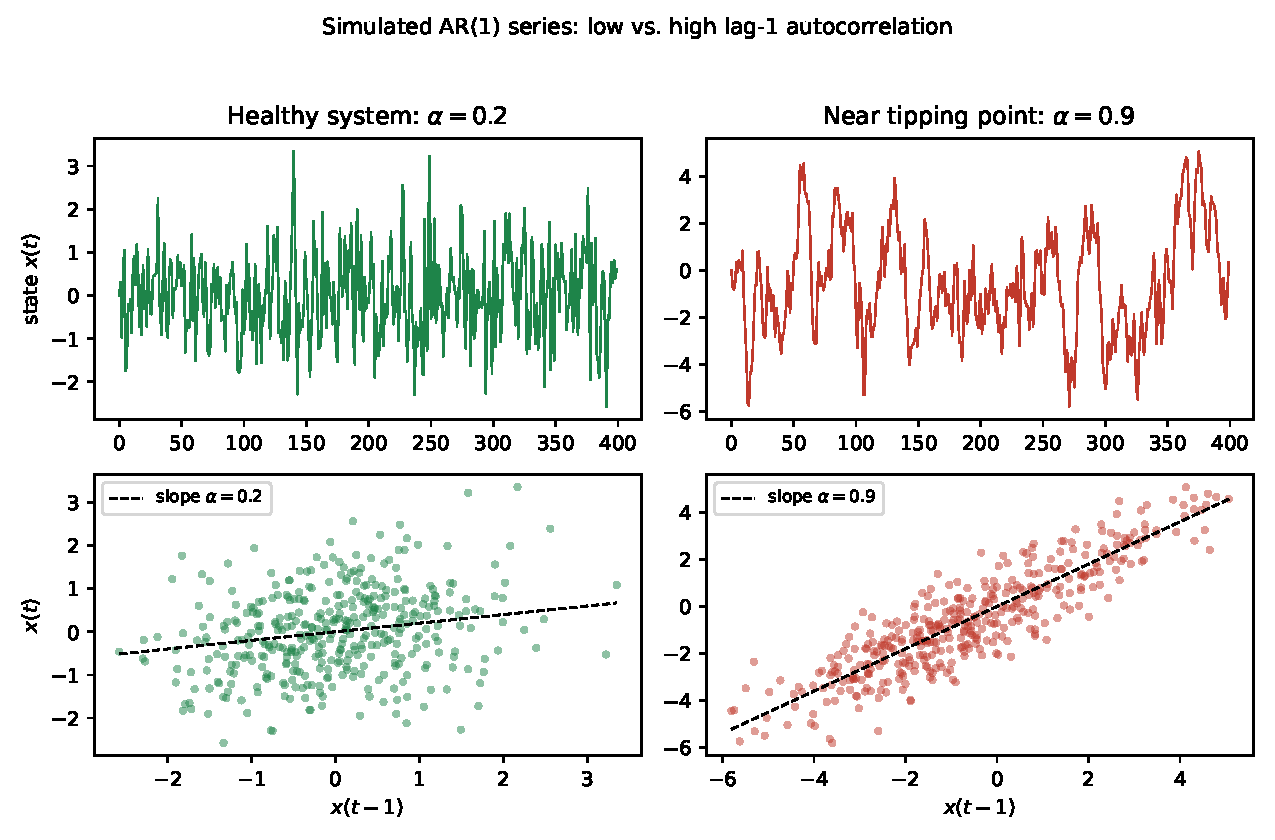
\includegraphics[width=0.85\textwidth]{figures/fig3_ar1_comparison.pdf}
    \caption{Two simulated AR(1) series ($\alpha=0.2$, far from any threshold, vs.\ $\alpha=0.9$, close to one) and their $x(t)$ vs.\ $x(t-1)$ scatter plots. The scatter-plot regression slope is $\alpha$ itself, and it visibly steepens as $\alpha\to1$.}
    \label{fig:3_2}
\end{figure}

\section{Classical Early Warning Signals vs.\ Deep Learning}
For over a decade, the standard way to look for early warning signals in real data has been the classical approach of \citet{dakos2012} and \citet{scheffer2009}: slide a window along the record, remove the slow background trend inside each window, measure the variance and lag-1 autocorrelation of what is left, and check whether those measurements rise steadily as the window moves toward the present. A steady rise, usually tested with a rank-correlation statistic called Kendall's $\tau$, is treated as a warning.

\subsection{How This Thesis Computes Variance and Autocorrelation}
\label{sec:actual_computation}
This thesis still computes variance and lag-1 autocorrelation the classical way, on the real cores, and it is worth stating exactly how, since the details matter later. For a window of $n$ values:

\begin{itemize}
    \item the variance is the ordinary spread of the values around their average: take each value's distance from the average, square it, add these up, and divide by $n-1$ (written $\frac{1}{n-1}\sum_i (x_i - \bar{x})^2$);
    \item the lag-1 autocorrelation is how strongly each value matches the value just before it: line the window up against a copy of itself shifted by one step, and take the correlation between the two.
\end{itemize}

Before either is computed, the slow background trend is removed by Gaussian smoothing: each point is replaced by the raw value minus a local weighted average of its neighbours, where nearby points count more than distant ones and ``nearby'' is set by a bandwidth of 900 years (\texttt{src/pangea\_cleaner.py}, config key \texttt{bandwidth\_years}). Each window covers half of the usable pre-transition segment, matching both \citet{dakos2012}'s convention and \citet{bury2021}'s own choice for this same anoxia evaluation -- stated directly in their methods, in the same sentence as the 900-year bandwidth: "EWS are computed using a rolling window of 0.5."

\subsection{How This Compares to Dakos and to Bury}
\label{sec:methodology_comparison}
This thesis's approach borrows from two earlier ones. Table~\ref{tab:methodology_comparison} lays out all three side by side. Being clear about what is borrowed and what is new matters more here than claiming this thesis's method is simply better.

\begin{table}[htbp]
\centering
\caption{Three approaches to the same underlying problem, compared on their actual methodological choices.}
\label{tab:methodology_comparison}
\begin{tabular}{p{2.6cm}p{3.6cm}p{3.6cm}p{3.6cm}}
\toprule
 & \textbf{Classical (Dakos et al.)} & \textbf{Bury et al. (2021)} & \textbf{This thesis} \\
\midrule
Detection & Hand-computed variance/AC1, trend read directly & Trained classifier's raw output & Trained classifier's raw output \\
Window & Half the series length & Classifier: full fixed-length input, no window. Classical EWS comparison (their Fig.\ 2): rolling window of 0.5, same anoxia evaluation & Half the segment (matches Dakos and Bury's own anoxia evaluation) for classical stats; fixed-length input for the classifier \\
Detrending & Gaussian/LOESS, human-chosen bandwidth & Lowess, span 0.2 (synthetic training data); Gaussian, 900 y (their own anoxia evaluation) & Same Gaussian, 900 y, matching Bury et al.'s own anoxia-evaluation method exactly \\
Bifurcation type & Cannot determine & In principle, via 4-class output & Same 4-class output, but cross-model reliability of the type read is explicitly measured (Chapter~\ref{ch:results}) \\
Significance test & Kendall's $\tau$ trend test & AR(1) null surrogates, AUC & Same AR(1) surrogate method as Bury, same fit-on-first-20\% convention \\
\bottomrule
\end{tabular}
\end{table}

Three of the choices in the last column are taken directly from earlier work, and it would be wrong to present them as new. The AR(1) surrogate test (described just below) copies the exact procedure from \citet{bury2021}'s own published code. The half-length window matches the long-standing convention of \citet{dakos2012} -- and, like the bandwidth below, it is also \citet{bury2021}'s own stated choice for their classical-EWS comparison on this same anoxia data, not only Dakos's. Their methods give both numbers in the same sentence: "smoothing the data with a Gaussian kernel with a bandwidth of 900 y, and EWS are computed using a rolling window of 0.5." Matching both here keeps this thesis's real-data preprocessing identical to theirs, on the same cores.

The reasoning for keeping that bandwidth fixed in years, rather than set as a fraction of each segment's length, is still worth stating, even though the number itself is inherited. After the sapropel ages were corrected (Chapter~\ref{ch:data}, Section~\ref{sec:label_correction}), the real segments range from about 100 to 650 data points -- a wider spread than either Bury et al. or \citet{dakos2012} needed to reconcile with one fixed bandwidth. A bandwidth set as a fraction of length would smooth each sapropel over a different span of real time, which makes no physical sense: the slow process being removed (orbital forcing) runs on the same timescale no matter how many data points a core happens to contain. A fixed 900-year bandwidth removes the same amount of slow trend from every segment, whatever its length.

One choice in the table is this thesis's own: keeping the classical variance and autocorrelation only as a support for the surrogate test, not as the detector. Unlike \citet{dakos2012}, this thesis does not read the rising trend in those numbers as the answer -- the answer comes from the trained classifiers, and the classical numbers are computed only to build the null comparison described next.

Whether the overall combination is ``better'' than either earlier approach is not a claim this thesis makes in general terms. What it can say from its own results (Chapter~\ref{ch:results}) is narrower: judged against the same AR(1) surrogate test that both Dakos and Bury use, the trained classifiers tell real pre-transition data apart from matched noise clearly better than chance on the corrected cores. But which bifurcation type they name is not consistent from one architecture to the next -- a gap the classical method cannot even attempt, and that Bury's own published work did not measure.

\subsection{Testing Significance Against a Null Model}
\label{sec:ar1_surrogates}
A rising Kendall's $\tau$ on its own is not enough, because a short, noisy record can drift upward just by chance. The standard safeguard is to compare the real record against many fake records built to have the same background noise but no approaching tipping point, and only accept the signal if the real record's trend is stronger than almost all of the fakes.

This thesis's evaluation on the real cores does exactly this (\texttt{testing/evaluate.py}), and it is worth being precise, because this is the one place where the classical theory in this chapter and the machine-learning evaluation later are the same calculation. For each real pre-transition segment: fit an AR(1) model to just the earliest 20\% of it -- the calmest part, least likely to already be slowing down, the same 20\% choice \citet{bury2021}'s own code uses -- and set the noise size from the fitted $\alpha$ and the segment's variance, using $\sigma_\epsilon = \sqrt{\text{Var}(y)\,(1-\alpha^2)}$ (the variance formula from Section~\ref{sec:ar1_model}, rearranged). Generate ten fake series from that fitted model. Run every trained classifier on the real segment and on its ten fakes. The AUC score (Chapter~\ref{ch:methodology}, Section~\ref{sec:evaluation_metrics}) then measures how well the classifier separates the real data from the matched fakes -- if it cannot, its output on the real data means nothing, however confident it looks.

\subsection{Limitations of the Classical Approach}
The classical approach has three well-known weak points. First, the window length is a hand-picked choice with real consequences: too short and the variance and autocorrelation estimates are themselves so noisy they drown the signal (this exact problem, and its fix, is in Chapter~\ref{ch:data}, Section~\ref{sec:label_correction}); too long and the window blurs over the fast dynamics right before the tipping point. Second, the detrending step can do harm as well as good -- the wrong filter can put a false rising trend into the leftover data by itself. Third, the classical method is one-dimensional: it can say that something is changing, but never which type of bifurcation is causing it, because Fold and Transcritical look identical through variance and autocorrelation alone (Section~\ref{sec:fold_transcritical_challenge}).

\subsection{The Deep Learning Response}
These weak points are what pushed this thesis toward deep learning and modern time series classification, learned from the large synthetic training set in Chapter~\ref{ch:data} instead of a person choosing a window length and a detrending filter by hand. The deep-learning models (CNN-LSTM and InceptionTime, among others) read the raw residual series directly. The classical time series classifiers (MiniRocket and WEASEL2, among others) read the raw series plus four engineered channels built on top of it, including the variance growth ratio from Section~\ref{sec:fold_transcritical_challenge}, so those models are handed an input designed to separate Fold from Transcritical directly; the deep-learning models are left to work that difference out for themselves from the raw series alone. The models themselves are the subject of Chapter~\ref{ch:methodology}.
